\section{Метод Гаусса решения систем линейных алгебраических уравнений. Алгоритм ортогонализации Грама–Шмидта.}

\subsection*{Метод Гаусса решения систем линейных алгебраических уравнений}

К точным методам решения системы $A\mathbf{x}=\mathbf{b}$ линейных алгебраических
уравнений (СЛАУ) относятся алгоритмы, которые при отсутствии ошибок
округления позволяют точно вычислить искомый вектор $\mathbf{x}$. Если число
ненулевых элементов матрицы имеет порядок $n^2$, то большинство такого
рода алгоритмов позволяет найти решение за $\bigO(n^3)$ арифметических
действий. Данная оценка, а также необходимость хранения всех элементов
матрицы в памяти машины, накладывают существенное ограничение
на область применимости точных методов. Однако, для решения задач не
очень большой размерности (от $10^3$ до $10^4$) в большинстве случаев разумно
применение точных алгоритмов. Отметим, что при численном решении задач
математической физики часто требуется обращать матрицы блочнодиагонального
вида. В этом случае удается построить точные методы с
меньшим по порядку числом арифметических действий. К таким алгоритмам относятся метод прогонки, стрельбы, Фурье (базисных функций).

Метод исключения Гаусса является наиболее известным из точных
методов, применяемых для задач с матрицами общего вида. В предположении, что
коэффициент $a_{11}\neq0$, в первом шаге уравнения исходной системы заменяются на
следующие
\[\left\{
  \begin{aligned}
     & x_1+\sum_{j=2}^n\frac{a_{1j}}{a_{11}}x_j=\frac{b_1}{a_{11}}                                                \\
     & \sum_{j=2}^nx_j\left(a_{ij}-\frac{a_{i1}}{a_{11}}a_{1j}\right)=b_i-\frac{b_1}{a_{11}}a_{i1},\ i=2,\ldots,n
  \end{aligned}
  \right.\]

В матричном виде при $n=3$ такой переход выглядит следующим образом.
Обозначим $A^{(0)}\equiv A$, $\mathbf{b}^{(0)}\equiv \mathbf{b}$
\[
  A^{(0)}\mathbf{x}=\mathbf{b}^{(0)}\Leftrightarrow
  \left(\begin{array}{ccc|c}
      1 & \frac{a_{12}}{a_{11}}              & \frac{a_{13}}{a_{11}}              & \frac{b_1}{a_{11}}             \\
      0 & a_{22}-\frac{a_{12}}{a_{11}}a_{21} & a_{23}-\frac{a_{12}}{a_{11}}a_{21} & b_{2}-\frac{b_1}{a_{11}}a_{21} \\
      0 & a_{32}-\frac{a_{12}}{a_{11}}a_{31} & a_{33}-\frac{a_{12}}{a_{11}}a_{31} & b_{3}-\frac{b_1}{a_{11}}a_{31}
    \end{array}\right)=:
  \left(\begin{array}{ccc|c}
      1 & \overline{a_{12}} & \overline{a_{13}} & \overline{b_{1}} \\
      0 & \overline{a_{22}} & \overline{a_{23}} & \overline{b_{2}} \\
      0 & \overline{a_{32}} & \overline{a_{33}} & \overline{b_{3}}
    \end{array}\right)\Leftrightarrow A^{(1)}\mathbf{x}=\mathbf{b}^{(1)}
\]
то есть первое уравнение делится на $a_{11}$, а затем, умноженное на соответствующий
коэффициент $a_{i1}$, вычитается из последующих уравнений. В полученной
системе $A^{(1)}\mathbf{x}=\mathbf{b}^{(1)}$ неизвестное $x_1$ оказывается исключенным
из всех уравнений, кроме первого. Далее, при условии, что коэффициент
$a_{22}^{(1)}$ матрицы $A^{(1)}$ отличен от нуля, исключаем $x_2$ из всех уравнений кроме
первого и второго, и т.д.
\[
  A^{(1)}\mathbf{x}=\mathbf{b}^{(1)}\rightarrow
  \left(\begin{array}{ccc|c}
      1 & \overline{a_{12}} & \overline{a_{13}}                                                              & \overline{b_{1}}                                                             \\
      0 & 1                 & \frac{\overline{a_{23}}}{\overline{a_{22}}}                                    & \frac{\overline{b_{2}}}{\overline{a_{22}}}                                   \\
      0 & 0                 & \overline{a_{33}}-\frac{\overline{a_{23}}}{\overline{a_{22}}}\overline{a_{32}} & \overline{b_{3}}-\frac{\overline{b_{2}}}{\overline{a_{22}}}\overline{a_{32}}
    \end{array}\right)=:
  \left(\begin{array}{ccc|c}
      1 & \widehat{a_{12}} & \widehat{a_{13}} & \widehat{b_{1}} \\
      0 & 1                & \widehat{a_{23}} & \widehat{b_{2}} \\
      0 & 0                & \widehat{a_{33}} & \widehat{b_{3}}
    \end{array}\right)\Leftrightarrow A^{(2)}\mathbf{x}=\mathbf{b}^{(2)}
\]
В итоге получим систему $A^{(n)}\mathbf{x}=\mathbf{b}^{(n)}$ с верхнетреугольной матрицей.
\[
  A^{(2)}\mathbf{x}=\mathbf{b}^{(2)}\rightarrow
  \left(\begin{array}{ccc|c}
      1 & \widehat{a_{12}} & \widehat{a_{13}} & \widehat{b_{1}}                          \\
      0 & 1                & \widehat{a_{23}} & \widehat{b_{2}}                          \\
      0 & 0                & 1                & \frac{\widehat{b_{3}}}{\widehat{a_{33}}}
    \end{array}\right)\Leftrightarrow A^{(3)}\mathbf{x}=\mathbf{b}^{(3)}
\]
Данная последовательность вычислений называется \textit{прямым ходом метода Гаусса}.
Из последнего уравнения приведенной системы определяем компоненту решения $\mathbf{x}$.
Далее подставляем $x_n$ в $(n-1)$-е уравнение, находим $x_{n-1}$ и т.д.
Соответствующая последовательность вычислений называется \textit{обратным ходом Гаусса}.
\[
  \left(\begin{array}{ccc|c}
      1 & \widehat{a_{12}} & \widehat{a_{13}} & \widehat{b_{1}}                          \\
      0 & 1                & \widehat{a_{23}} & \widehat{b_{2}}                          \\
      0 & 0                & 1                & \frac{\widehat{b_{3}}}{\widehat{a_{33}}}
    \end{array}\right)\rightarrow
  \left(\begin{array}{ccc|c}
      1 & 0 & 0 & \widehat{b_{1}} - \frac{\widehat{b_{3}}}{\widehat{a_{33}}}\widehat{a_{13}} - \left(\widehat{b_{2}} - \frac{\widehat{b_{3}}}{\widehat{a_{33}}}\widehat{a_{23}}\right)\widehat{a_{12}} \\
      0 & 1 & 0 & \widehat{b_{2}} - \frac{\widehat{b_{3}}}{\widehat{a_{33}}}\widehat{a_{23}}                                                                                                           \\
      0 & 0 & 1 & \frac{\widehat{b_{3}}}{\widehat{a_{33}}}
    \end{array}\right)
\]

Если на $k$-м шаге прямогохода коэффициeнтa $a_{kk}^{(k-1)}$ равен нулю,
тогда $k$-я строка уравнения переставляется с произвольной $l$-й строкой,
$l>k$ с ненулевым коэффициентом $a_{lk}^{(k-1)}$ при $x_k$.
Такая строка всегда найдется, если $\det(A)\neq0$.

Если на $k$-м шаге прямого хода диагональный элемент $a_{kk}^{(k-1)}$ отличен
от нуля, но имеет малое абсолютное значение, то коэффициенты очередной матрицы
$A^{(k)}$ будут вычислены с большой абсолютной погрешностью.
Это может существенно исказить найденный ответ. Поэтому при практической
реализации метода Гаусса следует на каждом шаге прямого хода переставлять на
$k$-е место строку с максимальным по модулю элементом $a_{lk}^{(k-1)}$ среди
всех $l\geq k$. Такая необходимая при расчетах модификация назвается
методом Гаусса с частичным выбором главного элемента. Данный
алгоритм позволяет гарантированно найти приближенное решение $\mathbf{x}$ с малой
нормой невязки $\dfrac{\norm{\mathbf{b}-A\tilde{\mathbf{x}}}}{\norm{\tilde{\mathbf{x}}}}$, но, возможно,
с большой нормой ошибки $\norm{\mathbf{x}-\tilde{\mathbf{x}}}$.


\begin{example}
  Пример нахождения решения СЛАУ методом Гаусса с выбором главного элемента
  по столбцу.
  \[
    \left(\begin{array}{ccc|c}
        1.00 & 2.00 & 3.00 & 3.00 \\
        3.00 & 1.00 & 2.00 & 6.00 \\
        2.00 & 3.00 & 1.00 & 9.00
      \end{array}\right)\rightarrow
    \left(\begin{array}{ccc|c}
        3.00 & 1.00 & 2.00 & 6.00 \\
        1.00 & 2.00 & 3.00 & 3.00 \\
        2.00 & 3.00 & 1.00 & 9.00
      \end{array}\right)\rightarrow
    \left(\begin{array}{ccc|c}
        1.00 & 0.33 & 0.67 & 2.00 \\
        1.00 & 2.00 & 3.00 & 3.00 \\
        2.00 & 3.00 & 1.00 & 9.00
      \end{array}\right)\rightarrow
  \]
  \[
    \left(\begin{array}{ccc|c}
        1.00 & 0.33 & 0.67  & 2.00 \\
        0.00 & 1.67 & 2.33  & 1.00 \\
        0.00 & 2.33 & -0.33 & 5.00
      \end{array}\right)\rightarrow
    \left(\begin{array}{ccc|c}
        1.00 & 0.33 & 0.67  & 2.00 \\
        0.00 & 2.33 & -0.33 & 5.00 \\
        0.00 & 1.67 & 2.33  & 1.00
      \end{array}\right)\rightarrow
    \left(\begin{array}{ccc|c}
        1.00 & 0.33 & 0.67  & 2.00 \\
        0.00 & 1.00 & -0.14 & 2.14 \\
        0.00 & 1.67 & 2.33  & 1.00
      \end{array}\right)\rightarrow
  \]
  \[
    \left(\begin{array}{ccc|c}
        1.00 & 0.33 & 0.67  & 2.00  \\
        0.00 & 1.00 & -0.14 & 2.14  \\
        0.00 & 0.00 & 2.57  & -2.57
      \end{array}\right)\rightarrow
    \left(\begin{array}{ccc|c}
        1.00 & 0.33 & 0.67  & 2.00  \\
        0.00 & 1.00 & -0.14 & 2.14  \\
        0.00 & 0.00 & 2.57  & -2.57
      \end{array}\right)\rightarrow
    \left(\begin{array}{ccc|c}
        1.00 & 0.33 & 0.67  & 2.00  \\
        0.00 & 1.00 & -0.14 & 2.14  \\
        0.00 & 0.00 & 1.00  & -1.00
      \end{array}\right)\rightarrow
  \]
  \[
    \left(\begin{array}{ccc|c}
        1.00 & 0.33 & 0.00 & 2.67  \\
        0.00 & 1.00 & 0.00 & 2.00  \\
        0.00 & 0.00 & 1.00 & -1.00
      \end{array}\right)\rightarrow
    \left(\begin{array}{ccc|c}
        1.00 & 0.00 & 0.00 & 2.00  \\
        0.00 & 1.00 & 0.00 & 2.00  \\
        0.00 & 0.00 & 1.00 & -1.00
      \end{array}\right)\rightarrow
    \left(\begin{array}{ccc|c}
        1.00 & 0.00 & 0.00 & 2.00  \\
        0.00 & 1.00 & 0.00 & 2.00  \\
        0.00 & 0.00 & 1.00 & -1.00
      \end{array}\right)
  \]
\end{example}

\begin{lemma}
  Реализация прямого и обратного хода метода Гаусса требует
  порядка $\frac{2}{3}n^3$ и $n^2$ арифметических действий соответственно.
\end{lemma}
\begin{proof}$ $\newline
  \begin{minipage}{.4\linewidth}
    \[\underset{\mbox{\Large $n\times n$}}{{\left(\begin{array}{c|ccc}
                1      &  &                                 & \\
                \hline
                0      &  &                                 & \\
                \vdots &  & \mbox{\Large$(n-1)\times(n-1)$} & \\
                0      &  &                                 & \\
              \end{array}\right)}}\]
  \end{minipage}\hfill
  \begin{minipage}{.5\linewidth}
    За первый шаг прямого хода метода Гаусса мы делаем $n^2$ операций сложения и умножения:
    первый столбец зануляем, остальные умножаем на соответствующие коэффициенты.
    За каждый следующий шаг метода мы будем работать с меньшим квадратом $(n-1)\times(n-1)$.
  \end{minipage}

  Таким образом, суммарно количество одной из операций за прямой ход метода Гаусса достигнет
  \[n^2+(n-1)^2+\ldots+1^2=\sum_{k=1}^nk^2\]
  Посчитаем это значение двумя способами:
  \[\begin{aligned}
      (k+1)^3=k^3+3k^2+3k+1        \\
      2^3=1^3+3\cdot 1^2+3\cdot1+1 \\
      3^3=2^3+3\cdot 2^2+3\cdot2+1 \\
      \ldots                       \\
      (n+1)^3=n^3+3\cdot n^2+3\cdot n+1
    \end{aligned}\Rightarrow
    \begin{aligned}
      \sum_{k=2}^{n+1}k^3=\sum_{k=1}^{n}k^3+3\left(\sum_{k=1}^{n}k^2\right)+3\left(\sum_{k=1}^{n}k\right)+n \\
      (n+1)^3 = 1 + 3\left(\sum_{k=1}^{n}k^2\right)+3\frac{(n+1)}{2}n+n                                     \\
      3\left(\sum_{k=1}^{n}k^2\right)=\frac{(n+1)(2n^2+4n-3n)}{2}                                           \\
      \sum_{k=1}^{n}k^2=\frac{n(n+1)(2n+1)}{6}\approx\frac{n^3}{3}
    \end{aligned}
  \]
  \begin{minipage}{0.3\linewidth}
    \centering
    \tikzsetnextfilename{24/ApproxSumOfSquares}
    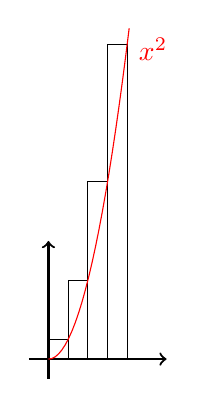
\begin{tikzpicture}[scale=0.25]
      \draw[thick,->] (0,-1) -- (0,6);
      \draw[thick,->] (-1,0) -- (6,0);
      \draw (0,0) rectangle (1,1);
      \draw (1,0) rectangle (2,4);
      \draw (2,0) rectangle (3,9);
      \draw (3,0) rectangle (4,16);
      \draw [domain=0:4.1, color=red] plot (\x,\x*\x) node[anchor=north west]{$x^2$};
    \end{tikzpicture}
  \end{minipage}\hfill
  \begin{minipage}{0.7\linewidth}
    Получим это значение иначе. Представим эту сумму как площадь следующих фигур.
    Заметим, что искомое значение является формулой вычисления интеграла
    через прямоугольник по крайней точке.
    \[\sum_{k=1}^{n}1\cdot k^2\approx \int_0^nx^2dx=\frac{n^3}{3}\]
  \end{minipage}

  За первый шаг обратного хода метода Гаусса мы делаем 1 операцию сложения и умножения:
  подставляем $x_{n}$, умножаем его на $a_{n-1n}$ и вычитаем из $b_{n-1}$.
  За каждый следующий шаг метода мы будем подставлять все предыдущие $x_i$
  умножать на соответствующие $a_{ij}$ и вычитать из соответствующего $b_i$.
  В итоге общее количество одной арифметической операции
  \[1+2+\ldots+(n-1)=(n-1)\frac{1+n-1}{2}=\frac{n^2-n}{2}\approx \frac{n^2}{2}\]
\end{proof}

\begin{theorem}
  Пусть матрица $A_{kk}^{(k-1)}$ не требует перестановок $\forall\ k=1,\ldots,n$.
  Тогда алгоритм Гаусса представим в виде
  \[C_n\ldots C_2'C_2C_1'C_1Ax=C_n\ldots C_1'C_1b\]
  где $C_i$ и $C_i'$ матрицы вида
  \[C_i=\left(\begin{array}{ccccc}
        1 &        &                       &        & 0 \\
          & \ddots &                       &        &   \\
          &        & (a_{ii}^{(i-1)})^{-1} &        &   \\
          &        &                       & \ddots &   \\
        0 &        &                       &        & 1 \\
      \end{array}\right);\quad
    C_i'=\left(\begin{array}{cccccccc}
        1 &        &   &                    &   &        &        & 0 \\
          & \ddots &   &                    &   &        &        &   \\
          &        & 1 &                    &   &        &        &   \\
          &        &   & 1                  &   &        &        &   \\
          &        &   & -a^{(i-1)}_{i+1,i} & 1 &        &        &   \\
          &        &   & -a^{(i-1)}_{i+2,i} & 0 & \ddots &        &   \\
          &        &   & \vdots             &   &        & \ddots &   \\
        0 &        &   & -a^{(i-1)}_{n,i}   &   &        &        & 1 \\
      \end{array}\right)\quad
  \]
\end{theorem}
\begin{proof}
  Доказывается непосредственной проверкой, что на $i$-ом
  шаге матрица $A^{(i-1)}$ при умножении слева на $C_i$ нормирует
  первый элемент, а при умножении слева на $C_i'$ из $i+1$ строки
  вычитается $i$-ая строка умноженная на $-a_{i+1,i}^{(i-1)}$.
\end{proof}

Метод Гаусса по сути соответствует разложению исходной матрицы
$A$ на произведение нижнетреугольной $L$ и верхнетреугольной $R$.
Действительно, $C=AR,\ C\defeq C_n\ldots C_1'C_1$ - нижнетреугольная матрица,
$R$ - верхнетреугольная матрица с единичной диагональю.
Поэтому $A = LR$, где $L=C^{-1}$.

Прямой ход метода Гаусса с частичным выбором главного элемента
соответствует последовательному умножению исходной системы на
некоторые диагональные матрицы $C_k$, нижнетреугольные матрицы
$C_k'$ и матрицы перестановок $P_k^{ij}$. При этом задание матриц
$C_k$, $C_k'$ совпадают с матриц метода Гаусса, матрицы $P_k^{ij}$ получаются из единичной матрицы $I$
некоторой перестановкой строк.

\[P_k^{ij}=\left(\begin{array}{ccccccc}
      1 &        &   &        &   &        & 0 \\
        & \ddots &   &        &   &        &   \\
        &        & 0 &        & 1 &        &   \\
        &        &   & \ddots &   &        &   \\
        &        & 1 &        & 0 &        &   \\
        &        &   &        &   & \ddots &   \\
      0 &        &   &        &   &        & 1 \\
    \end{array}\right)
  \begin{array}{c}
    \\
    \\
    i \\
    \\
    j \\
    \\
    \\
  \end{array}
\]

Такой подход гарантирует, что метод находит приближенное решение с
малой относительной невязкой (но, возможно, большой ошибкой). Метод
Гаусса с выбором на каждом шаге наибольшего элемента по всей подматрице
на практике почти не применяется, хотя имеются немногочисленные
примеры, когда он дает качественное улучшение.

Отметим, что для невырожденной матрицы $A$ существуют матрицы перестановок
$P_1$ и $P_2$, нижняя треугольная матрица $L$ и верхнетреугольная
$R$ такие, что $P_1AP_2=LR$. При этом достаточно оодной из матриц
$P_i$. Умножение $A$ на матрицу $P_i$ слева переставляет строки исходной
матрицы, а умножение на $P_2$ справа  столбцы. Для того чтобы матрица
имела $LR$-разложение, необходимо и достаточно, чтобы все ее ведущие подматрицы
(в том числе и $A$) были невырожденные.

\newpage
\subsection*{Алгоритм ортогонализации Грама-Шмидта}

Хотим по набору линейно-независимых векторов $<\mathbf{a}_1,\ldots,\mathbf{a}_n>$ получить
подпространство $<\mathbf{q}_1,\ldots,\mathbf{q}_n>$ такое, что $(\mathbf{q}_i,\mathbf{q}_j)=\delta_{ij}$.

Суть метода Грама-Шмидта состоит во взятии первого ортогонального вектора
равным первому исходному вектору и построении каждого нового ортогонального
вектора равным текущему исходному вектору, скорректированному на величины
проекций текущего вектора на предыдущие ортогональные векторы.

\[
  \begin{array}{lclr}
    \widetilde{\mathbf{q}}_1 & =     & \mathbf{a}_1                                                                                   & \mathbf{q}_1=\widetilde{\mathbf{q}}_1/\norml{\widetilde{q}_1}{2} \\
    \widetilde{\mathbf{q}}_2 & =     & \mathbf{a}_2-(\mathbf{q}_1, \mathbf{a}_2)\mathbf{q}_1                                          & \mathbf{q}_2=\widetilde{\mathbf{q}}_2/\norml{\widetilde{q}_2}{2} \\
    \widetilde{\mathbf{q}}_3 & =     & \mathbf{a}_3-(\mathbf{q}_2, \mathbf{a}_3)\mathbf{q}_2-(\mathbf{q}_1, \mathbf{a}_3)\mathbf{q}_1 & \mathbf{q}_3=\widetilde{\mathbf{q}}_3/\norml{\widetilde{q}_3}{2} \\
                             & \dots &                                                                                                &                                                                  \\
    \widetilde{\mathbf{q}}_n & =     & \mathbf{a}_n-\sum_{i=1}^{n-1}(\mathbf{q}_i, \mathbf{a}_n)\mathbf{q}_i                          & \mathbf{q}_n=\widetilde{\mathbf{q}}_n/\norml{\widetilde{q}_n}{2}
  \end{array}
\]

\begin{theorem}
  Вектора $\{\mathbf{q}_i\}_{i=1}^n$ ортонормальны: $(\mathbf{q}_i,\mathbf{q}_j)=\delta_{ij}$.
\end{theorem}
\begin{proof}
  Проведем доказательство с помощью индукции
  \begin{itemize}
    \item База:
          \[(\mathbf{q}_1, \mathbf{q}_1)=\left(\frac{\mathbf{a}_1}{\norml{\mathbf{a}_1}{2}}, \frac{\mathbf{a}_1}{\norml{\mathbf{a}_1}{2}}\right)=\frac{1}{\norml{\mathbf{a}_1}{2}^2}(\mathbf{a}_1,\mathbf{a}_1)=1\]
          \[(\mathbf{q}_1, \mathbf{q}_2)=\left(\frac{\mathbf{a}_1}{\norml{\mathbf{a}_1}{2}}, \frac{\mathbf{a}_2-(\mathbf{q}_1, \mathbf{a}_2)\mathbf{q}_1}{\norml{\mathbf{a}_2-(\mathbf{q}_1, \mathbf{a}_2)\mathbf{q}_1}{2}}\right)=\frac{\left(\mathbf{a}_1, (\mathbf{a}_1,\mathbf{a}_1)\mathbf{a}_2-(\mathbf{a}_1, \mathbf{a}_2)\mathbf{a}_1\right)}{\norml{\mathbf{a}_1}{2}\norml{(\mathbf{a}_1,\mathbf{a}_1)\mathbf{a}_2-(\mathbf{a}_1, \mathbf{a}_2)\mathbf{a}_1}{2}}=\]
          \[=\frac{\left(\mathbf{a}_1, (\mathbf{a}_1,\mathbf{a}_1)\mathbf{a}_2\right)-\left(\mathbf{a}_1, (\mathbf{a}_1, \mathbf{a}_2)\mathbf{a}_1\right)}{\norml{\mathbf{a}_1}{2}\norml{(\mathbf{a}_1,\mathbf{a}_1)\mathbf{a}_2-(\mathbf{a}_1, \mathbf{a}_2)\mathbf{a}_1}{2}}=\frac{(\mathbf{a}_1,\mathbf{a}_1)(\mathbf{a}_1, \mathbf{a}_2)-(\mathbf{a}_1, \mathbf{a}_2)(\mathbf{a}_1, \mathbf{a}_1)}{\norml{\mathbf{a}_1}{2}\norml{(\mathbf{a}_1,\mathbf{a}_1)\mathbf{a}_2-(\mathbf{a}_1, \mathbf{a}_2)\mathbf{a}_1}{2}}=0\]
    \item Шаг индукции. Пусть предположение верно $\forall\ k < n$. Для упрощения выкладок рассмотрим ненормированный $\widetilde{\mathbf{q}_n}$.
          \[(\widetilde{\mathbf{q}_n}, \mathbf{q}_k)=(\mathbf{a}_n-\sum_{i=1}^{n-1}(\mathbf{q}_i, \mathbf{a}_n)\mathbf{q}_i, \mathbf{q_k})=(\mathbf{a}_n,\mathbf{q}_k)-\left(\sum_{i=1}^{n-1}(\mathbf{q}_i, \mathbf{a}_n)\mathbf{q}_i, \mathbf{q_k}\right)=(\mathbf{a}_n,\mathbf{q}_k)-(\mathbf{a}_n,\mathbf{q}_k)(\mathbf{q}_k,\mathbf{q}_k)=0\]
  \end{itemize}
\end{proof}

\subsection*{Модифицированный алгоритм ортогонализации Грама-Шмидта}
математически эквивалентен предыдущему, но более устойчив при наличии
вычислительной погрешности:
\[
  \begin{array}{lclr}
    \mathbf{q}_1 & =      & \mathbf{a}_1                                                   & \mathbf{q}_1=\mathbf{q}_1/\norml{q_1}{2} \\
    \mathbf{q}_2 & =      & \mathbf{a}_2                                                   &                                          \\
    \mathbf{q}_2 & =      & \mathbf{q}_2-(\mathbf{q}_1, \mathbf{q}_2)\mathbf{q}_1          & \mathbf{q}_2=\mathbf{q}_2/\norml{q_2}{2} \\
                 & \dots  &                                                                &                                          \\
    \mathbf{q}_n & =      & \mathbf{a}_n                                                   &                                          \\
    \mathbf{q}_n & =      & \mathbf{q}_n -(\mathbf{q}_1, \mathbf{q}_n)\mathbf{q}_1         &                                          \\
    \mathbf{q}_n & =      & \mathbf{q}_n -(\mathbf{q}_2, \mathbf{q}_n)\mathbf{q}_2         &                                          \\
                 & \ldots &                                                                &                                          \\
    \mathbf{q}_n & =      & \mathbf{q}_n -(\mathbf{q}_{n-1}, \mathbf{q}_n)\mathbf{q}_{n-1} & \mathbf{q}_n=\mathbf{q}_n/\norml{q_n}{2} \\
  \end{array}
\]

Вычислительная устойчивость достигается за счет вычитания уже наайденных
$\mathbf{q}_i$ из $\mathbf{a}_n$. В этом случае накопление погрешности при вычислении $\mathbf{q}_n$
из-за неточной ортогональности $\{\mathbf{q}_i\}$, $i<n$ происходит существенно медленнее.
